% Resultados principales: campaña final de 180 comandos del 26-10-2026.
% Revisión del 27-10-2026: comparación preliminar indicativa y correcciones de presentación.
% Se conserva una sola observación principal por caso-variante-modalidad.
\documentclass[a4paper,fleqn]{cas-dc}

\usepackage[T1]{fontenc}
\usepackage{iftex}
\ifPDFTeX\usepackage[utf8]{inputenc}\fi
\usepackage[authoryear,longnamesfirst]{natbib}
\usepackage[spanish,es-tabla,es-nodecimaldot,es-noshorthands]{babel}
\usepackage{amsmath,amssymb}
\usepackage{graphicx}
\usepackage{xcolor}
\usepackage{booktabs}
\usepackage{tabularx}
\usepackage{placeins}
\usepackage{xurl}
\usepackage{multirow}
\usepackage{algorithm}
\usepackage{algpseudocode}
\hypersetup{hypertexnames=false}

\newdefinition{definicion}{Definición}

\shorttitle{Programación automática de PLC mediante voz y LLM}
\shortauthors{Ochoa Zea y Chasi Pesantez}

\newcommand{\pend}[1]{\textbf{[PENDIENTE: #1]}}
\newcommand{\sinmedir}{\textemdash}

% Cargar UNA VEZ en el preámbulo, después de los demás paquetes.
% Ajustes de compatibilidad para cas-dc; no modifica la clase del tutor.
\usepackage{etoolbox}
\usepackage{icomma}
\urlstyle{tt}

% Encabezados en español por la indicación más reciente del autor.
% La plantilla CAS permite personalizar estos rótulos sin modificar sus archivos.
\newif\ifTitulosEnEspanol
\TitulosEnEspanoltrue
\ifTitulosEnEspanol
  \newcommand{\TituloIntroduccion}{Introducción}
  \newcommand{\TituloMetodos}{Materiales y métodos}
  \newcommand{\TituloResultados}{Resultados}
  \newcommand{\TituloDiscusion}{Discusión}
  \newcommand{\TituloConclusiones}{Conclusiones}
  \newcommand{\TituloDestacados}{Aspectos destacados}
  \newcommand{\TituloAgradecimientos}{Agradecimientos}
  \addto\captionsspanish{%
    \renewcommand{\abstractname}{Resumen}%
    \renewcommand{\refname}{Referencias}%
  }
  \AtBeginDocument{%
    \renewcommand{\abstractname}{Resumen}%
    \renewcommand{\refname}{Referencias}%
  }
\else
  \newcommand{\TituloIntroduccion}{Introduction}
  \newcommand{\TituloMetodos}{Materials and Methods}
  \newcommand{\TituloResultados}{Results}
  \newcommand{\TituloDiscusion}{Discussion}
  \newcommand{\TituloConclusiones}{Conclusions}
  \newcommand{\TituloDestacados}{Highlights}
  \newcommand{\TituloAgradecimientos}{Acknowledgements}
  \addto\captionsspanish{%
    \renewcommand{\abstractname}{Abstract}%
    \renewcommand{\refname}{References}%
  }
  \AtBeginDocument{%
    \renewcommand{\abstractname}{Abstract}%
    \renewcommand{\refname}{References}%
  }
\fi


% El BST CAS omite number en los artículos. Mostrar el número verificado de
% Jiang sin alterar volume/number en BibTeX ni modificar el archivo BST.
\newcommand{\TesisClaveBibliograficaActual}{}
\NewDocumentCommand{\TesisBibitemConClave}{o m}{%
  \def\TesisClaveBibliograficaActual{#2}%
  \IfNoValueTF{#1}
    {\TesisBibitemOriginal{#2}}
    {\TesisBibitemOriginal[#1]{#2}}%
}
\AtBeginEnvironment{thebibliography}{%
  \NewCommandCopy\TesisBibitemOriginal\bibitem
  \let\bibitem\TesisBibitemConClave
}
\providecommand{\bibinfo}[2]{#2}
\NewCommandCopy\TesisBibinfoOriginal\bibinfo
\RenewDocumentCommand{\bibinfo}{m m}{%
  \TesisBibinfoOriginal{#1}{#2}%
  \ifdefstring{\TesisClaveBibliograficaActual}{jiang2026survey}
    {\ifstrequal{#1}{volume}{(2)}{}}{}%
}


\setlength{\emergencystretch}{1em}
\tolerance=1000

\makeatletter
% Alinear arriba las páginas de flotantes de dos columnas, incluido el catálogo.
% El espacio elástico superior de LaTeX lo centraba pese a [t].
\setlength{\@dblfptop}{0pt}
\setlength{\@fptop}{0pt}

  % CAS superpone ARTICLE INFO en una caja de ancho cero. El pegamento
  % final permite la superposición sin un desbordamiento artificial.
  \ExplSyntaxOn
  % Usar etiqueta de correo en texto; no exigir thumbnails/cas-email.jpeg.
  \cs_if_exist:NT \g_stm_nologo_bool
    { \bool_gset_true:N \g_stm_nologo_bool }
  \cs_if_exist:cT { environment~Abstract~code }
    {
      \exp_args:Nc \patchcmd { environment~Abstract~code }
        { \hbox_to_wd:nn { \z@ } { \box \g_stm_key_box } }
        { \hbox_to_wd:nn { \z@ } { \box \g_stm_key_box \hss } }
        { }
        { \PackageWarning{ajustes-tesis}{No~se~aplico~el~ajuste~de~Abstract;~revisar~la~version~CAS} }
    }
  % No imprimir una nota ORCID vacía cuando no se suministraron datos.
  \cs_if_exist:NT \printorcid
    {
      \NewCommandCopy \thesis_original_printorcid: \printorcid
      \RenewDocumentCommand \printorcid { }
        { \seq_if_empty:NF \g_stm_orcid_seq { \thesis_original_printorcid: } }
    }
  \ExplSyntaxOff
\@ifclassloaded{cas-dc}{%
  % Las notas CAS usan footnotetext sin footnotemark. Asignar destinos
  % únicos conserva hyperref y evita anclas vacías o duplicadas.
  \NewCommandCopy\ThesisOriginalFirstPageNotes\printFirstPageNotes
  \RenewDocumentCommand\printFirstPageNotes{}{%
    \begingroup
    \NewCommandCopy\ThesisOriginalFootnoteText\footnotetext
    \RenewDocumentCommand\footnotetext{o +m}{%
      \stepcounter{Hfootnote}%
      \edef\Hy@footnote@currentHref{Hfootnote.\theHfootnote}%
      \IfNoValueTF{##1}
        {\ThesisOriginalFootnoteText{##2}}
        {\ThesisOriginalFootnoteText[##1]{##2}}%
    }%
    \ThesisOriginalFirstPageNotes
    \endgroup
  }%
}{}
\makeatother


\begin{document}
\let\WriteBookmarks\relax
\shortcites{zhuo2025bigcodebench}
\def\floatpagepagefraction{1}
\def\textpagefraction{.001}

\setcounter{topnumber}{3}
\setcounter{dbltopnumber}{3}
\setcounter{totalnumber}{5}
\renewcommand{\topfraction}{.95}
\renewcommand{\dbltopfraction}{.95}
% Fragmento para sustituir título, autores y afiliación en la plantilla CAS.
\title[mode=title]{Arquitectura para la programación automática de controladores lógicos programables mediante comandos de voz y modelos de lenguaje de gran tamaño aplicada a sistemas de automatización industrial}
% La declaración de financiamiento se incluye al final del artículo.
\author[1]{Henry Fernando {Ochoa Zea}}[orcid=0009-0006-7344-3680]
\cormark[1]
\ead{hochoaz@est.ups.edu.ec}
\author[1]{Paul Andres {Chasi Pesantez}}[orcid=0000-0002-4364-7483]
\affiliation[1]{organization={Universidad Politécnica Salesiana, Maestría en Automatización para la Industria 4.0},
city={Cuenca},country={Ecuador}}
\cortext[1]{Autor de correspondencia.}

\begin{abstract}
La programación de PLC requiere conservar los requisitos al interpretar instrucciones, asignar señales y generar código. Se presenta una arquitectura que recibe voz o texto en español, obtiene una interpretación estructurada mediante un modelo de lenguaje de gran tamaño (LLM) y construye localmente una representación intermedia y código SCL, con integración mediante TIA Openness. La versión final se evaluó con veinte casos discretos, tres variantes lingüísticas y tres modalidades: 180 comandos con interpretación LLM y un mapa I/O común. Las condiciones acústicas compartieron 60 locuciones y sus derivados con ruido a 10 dB. La evaluación utilizó TIA Portal V18 y S7-PLCSIM Advanced V5, con expectativas separadas del generador. Compilaron 58, 59 y 57 programas en texto, voz limpia y voz con ruido, respectivamente. Cada modalidad obtuvo 55/60 PASS (91,67\,\%); en total hubo siete fallos y ocho resultados sujetos a revisión. El WER global fue 4,79\,\% en voz limpia y 6,91\,\% con ruido. La igualdad de las tasas globales coexistió con diferencias entre comandos y no demuestra equivalencia entre modalidades. La trazabilidad permitió distinguir discrepancias de interpretación, asignación, tipado y comportamiento. La evidencia se limita al catálogo discreto y a las condiciones de simulación evaluadas.
\end{abstract}
\begin{highlights}[\TituloDestacados]

\item El LLM interpreta requisitos y el generador local construye la IR y el SCL.
\item Se evaluaron 180 comandos con un mapa I/O común y entradas acústicas pareadas.
\item Cada modalidad obtuvo 55 de 60 comandos conformes (91,67\,\%).
\item La evaluación distingue compilación, conformidad y resultados sujetos a revisión.


\end{highlights}
\begin{keywords}

% Pegar dentro del entorno keywords de la plantilla, si lo utiliza.
Controladores lógicos programables \sep Lenguaje natural \sep Modelos de lenguaje \sep Reconocimiento de voz \sep SCL \sep Control discreto


\end{keywords}
\maketitle

\section{\TituloIntroduccion}
\label{sec:intro}
Los controladores lógicos programables (PLC) implementan secuencias, enclavamientos y respuestas temporizadas cuya programación exige traducir requisitos de operación a señales y reglas ejecutables. La mantenibilidad del software constituye un problema durante la vida de máquinas y plantas \citep{vogelheuser2018maintainability}. El lenguaje natural facilita expresar esos requisitos; la voz añade una transformación acústica que puede alterar negaciones, símbolos o cantidades. La asistencia resulta útil cuando conserva el comportamiento solicitado y produce programas revisables.

La generación con modelos de lenguaje de gran tamaño (LLM) comprende datos, modelos y evaluación \citep{jiang2026survey}. Los benchmarks ejecutables generales, como BigCodeBench en Python, aportan criterios de seguimiento de instrucciones sin acreditar compatibilidad PLC \citep{zhuo2025bigcodebench}. En automatización, los enfoques basados en modelos, las extensiones orientadas a procesos y la traducción Python--ST organizan el comportamiento antes de ejecutarlo \citep{obermeier2015model,bashev2020post,zhao2024py2st}; la integración Gazebo-ROS vincula lógica y simulación \citep{kim2020gazebo}.

Los estudios iniciales de ChatGPT y modelos generales para PLC mostraron posibilidades y limitaciones de la generación desde descripciones \citep{koziolek2023chatgpt,tran2024universal}. Los enfoques posteriores incorporan especificaciones recuperadas, ajuste guiado por lógica y extracción de recursos \citep{koziolek2024rag,ren2025metaindux,boudribila2025requirements}. Identificar las señales de un requisito no basta para obtener un programa que cumpla el comportamiento esperado. Las evaluaciones mediante similitud, modelos y revisión humana responden además a criterios diferentes \citep{adnyana2026prompting}. AutoPLC y los agentes con recuperación de contexto acercan la generación a las herramientas del fabricante \citep{yang2025autoplc,kersting2025vendor}.

La comprobación externa permite distinguir el código plausible del comportamiento aceptable. LLM4PLC combina interacción, compilación y verificación SMV \citep{fakih2024llm4plc}. Agents4PLC relaciona requisitos y verificación de código, y SemaPLC incorpora contexto y trazas de ejecución \citep{liu2024agents4plc,tu2026semaplc}; las versiones consultadas de estos dos últimos son preprints. PLCverif, ESBMC-PLC+ y los análisis de GRAFCET aportan comprobaciones formales con alcances propios \citep{blanco2020plcverif,dantas2026esbmc,schnakenbeck2026comparison}. Los estímulos aplicados y el modelo de planta condicionan las pruebas conductuales \citep{ma2019plantfeatures}. La presencia de aserciones incorrectas en pruebas generadas con LLM y la separación de tareas y restricciones en PLCWorld resaltan la calidad del evaluador \citep{koziolek2024tests,kim2026plcworld}.

Whisper, OWSM y DGSRN constituyen antecedentes de reconocimiento multilingüe y en ruido \citep{radford2023whisper,peng2024owsm,peng2025owsm,wang2024dgsrn}. Las transcripciones pueden incorporar contenido ajeno a la señal \citep{koenecke2024careless}. Su aplicación a comandos PLC en español exige observar cómo las discrepancias se propagan desde el audio hasta el programa y su ejecución.

En los trabajos revisados no se identificó una evaluación que combine entrada de voz en español, condiciones acústicas pareadas, criterios conductuales separados del generador e integración Siemens. Esta brecha motiva estudiar la conservación del requisito a través de toda la cadena.

Este trabajo caracteriza una cadena voz/texto--LLM--PLC con mapa I/O autorizado, representación intermedia (IR), emisión SCL e integración Siemens. Su aporte es enlazar solicitud, interpretación, recursos, código, diagnósticos y trazas, y comparar las mismas variantes bajo tres modalidades. La Tabla~\ref{tab:comparativa} sitúa la propuesta frente a los antecedentes.

\begin{table*}[!tp]
\caption{Antecedentes relacionados con la generación, integración y evaluación de lógica PLC. Las tareas y criterios de aceptación difieren entre trabajos.}
\label{tab:comparativa}
\small
\begin{tabularx}{\textwidth}{@{}p{.20\textwidth} >{\raggedright\arraybackslash}X >{\raggedright\arraybackslash}X >{\raggedright\arraybackslash}X@{}}
\toprule Trabajo & Generación y contexto & Comprobación documentada & Relación con esta propuesta\\ \midrule
\citet{koziolek2023chatgpt} & GPT-4 y 100 prompts PLC/DCS en diez categorías & Estudio exploratorio de los programas obtenidos & Delimitar tareas y revisar el significado del código\\
\citet{tran2024universal} & Modelos generales y 21 ejemplos de programación PLC & CodeBERTScore, pass@k y tiempo de generación & Separar medidas del código y comprobación del comportamiento\\
\citet{koziolek2024rag} & Lenguaje natural y especificaciones de bloques & Compilación y simulación OpenPLC/OSCAT & Incorporar contexto técnico antes de emitir código\\
\citet{fakih2024llm4plc} & LLM e interacción con el usuario & Gramática, compilación, SMV y banco FischerTechnik & Combinar asistencia y comprobaciones externas\\
\citet{liu2024agents4plc} & Agentes y benchmark con especificaciones & Verificación a nivel de código & Relacionar requisito y criterio de aceptación\\
\citet{yang2025autoplc} & Planificación, recuperación de casos y bibliotecas del fabricante & Validación mediante TIA Portal y CODESYS & Integrar la generación con herramientas del fabricante\\
\citet{tu2026semaplc} & Contexto del proyecto & Compilación y comparación de trazas en ejecución & Conservar contexto y evidencia conductual\\
\citet{kim2026plcworld} & ST acoplado con una planta simulada & Cumplimiento de tareas y violaciones de restricciones; controles de referencia y contraejemplos & Comprobar el evaluador y separar comportamiento y restricciones\\
Este trabajo & Voz/texto en español, mapa I/O, IR y emisión SCL & Verificación local, TIA V18 y Oracle en PLCSIM Advanced & 180 comandos evaluados; tres modalidades y 165 conformes\\
\bottomrule
\end{tabularx}
\end{table*}

\textbf{Objetivo general.} Desarrollar una arquitectura de programación automática de PLC mediante comandos de voz y modelos de lenguaje de gran tamaño (LLM), capaz de generar y ejecutar código IEC 61131-3 en un entorno de simulación para aplicaciones de automatización industrial.

\textbf{Objetivos específicos.}
\begin{enumerate}
\item Analizar los requisitos funcionales y operativos necesarios para implementar una arquitectura de programación automática de PLC en un entorno simulado, a partir de comandos de voz y modelos de lenguaje (LLM).
\item Diseñar una plataforma que interprete comandos de voz en lenguaje natural y los traduzca en instrucciones semánticamente estructuradas para el modelo de lenguaje.
\item Implementar el sistema de generación automática de código IEC 61131-3 mediante modelos de lenguaje (LLM), incluyendo su ejecución directa en un simulador de PLC.
\item Validar el funcionamiento de la arquitectura propuesta mediante pruebas de generación, carga y ejecución de lógica PLC en un entorno simulado, con el fin de evaluar su desempeño y confiabilidad.
\end{enumerate}

La pregunta de investigación es: \textquestiondown{}en qué medida la arquitectura conserva los requisitos D01--D20 y cómo cambia su desempeño entre texto, voz limpia y voz con ruido? Las contribuciones comprenden el flujo interactivo con aclaraciones, la transformación trazable semántica--I/O--IR--SCL y su evaluación con entradas pareadas y un Oracle separado del generador.


\section{\TituloMetodos}
\label{sec:metodos}
Se desarrolló y evaluó una arquitectura de programación de lógica discreta en el entorno Siemens. La Tabla~\ref{tab:requisitos_arquitectura} vincula sus requisitos con comprobaciones observables; la Sección~\ref{sec:resultados} presenta la evidencia obtenida.

\begin{table*}[!tp]
\caption{Requisitos funcionales (RF) y operativos (RO) y criterio de comprobación.}
\label{tab:requisitos_arquitectura}
\small
\begin{tabularx}{\textwidth}{@{}l >{\raggedright\arraybackslash}X >{\raggedright\arraybackslash}X@{}}
\toprule ID & Requisito & Comprobación\\ \midrule
RF1 & Recibir texto o voz en español & Conservar entrada, audio y transcripción aplicables\\
RF2 & Interpretar intención, señales y parámetros & Validar semántica y contrastar expectativas del caso\\
RF3 & Gestionar información insuficiente & Registrar solicitud de aclaración y decisión\\
RF4 & Resolver recursos autorizados & Comprobar tipo, dirección, disponibilidad y permisos\\
RF5 & Construir IR y emitir SCL & Verificar declaraciones, bloques y requisitos\\
RF6 & Integrar y ejecutar & Registrar compilación, descarga y conexión RUN\\
RF7 & Conservar el comportamiento & Comparar trazas con expectativas e invariantes\\
RO1 & Aislar proyecto y recursos & Copiar el maestro y conservar mapa y asignación\\
RO2 & Mantener trazabilidad & Enlazar artefactos, incidencias y veredicto por comando\\
RO3 & Comparar modalidades pareadas & Asociar referencia, locución limpia y derivado ruidoso\\
\bottomrule
\end{tabularx}
\end{table*}

\subsection{Arquitectura e implementación}
\label{sec:arquitectura}
La cadena comprende entrada, reconocimiento de voz cuando corresponde, interpretación semántica, resolución I/O, IR, emisión SCL, verificación local e integración con TIA Openness (Figura~\ref{fig:arquitectura}). La interfaz reúne configuración, comando, resultados y consola (Figura~\ref{fig:interfaz_usuario}).

\begin{figure*}[!tp]
\centering
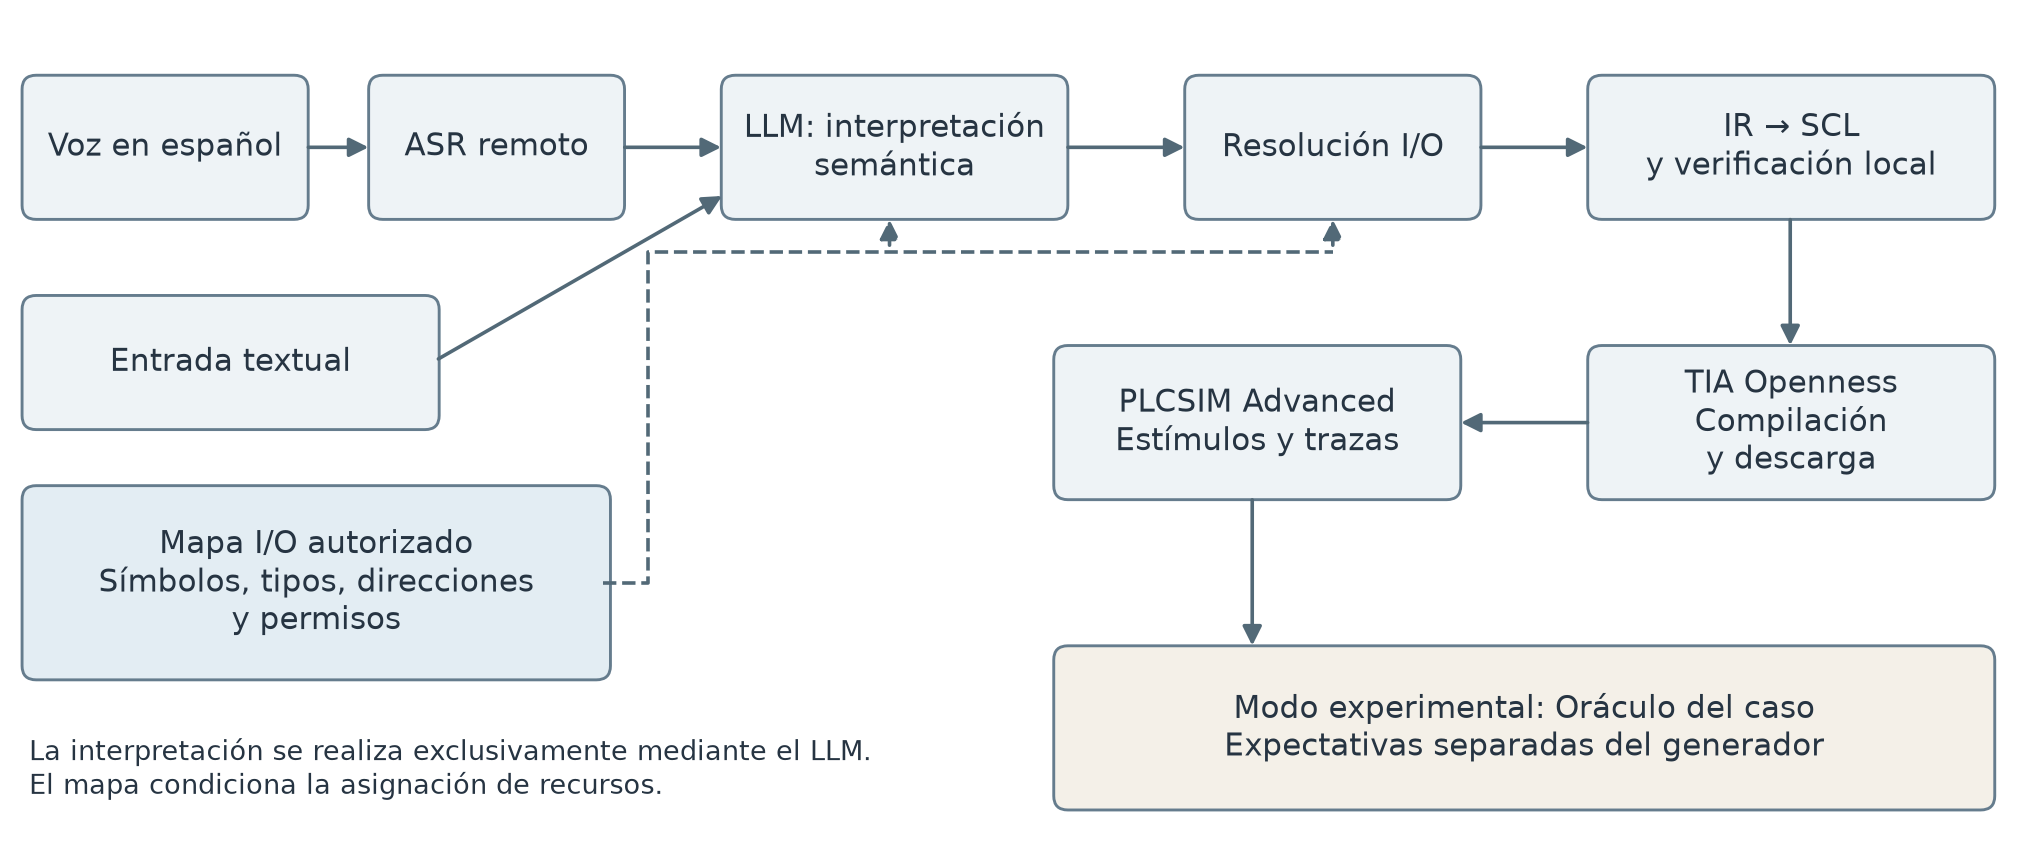
\includegraphics[width=\textwidth]{Graficos/arquitectura_voz_llm_plc.png}
\caption{Flujo voz/texto--LLM--PLC. El mapa delimita recursos y la entrada textual omite ASR; el destino experimental fue PLCSIM Advanced.}
\label{fig:arquitectura}
\end{figure*}
\begin{figure*}[!tp]
\centering
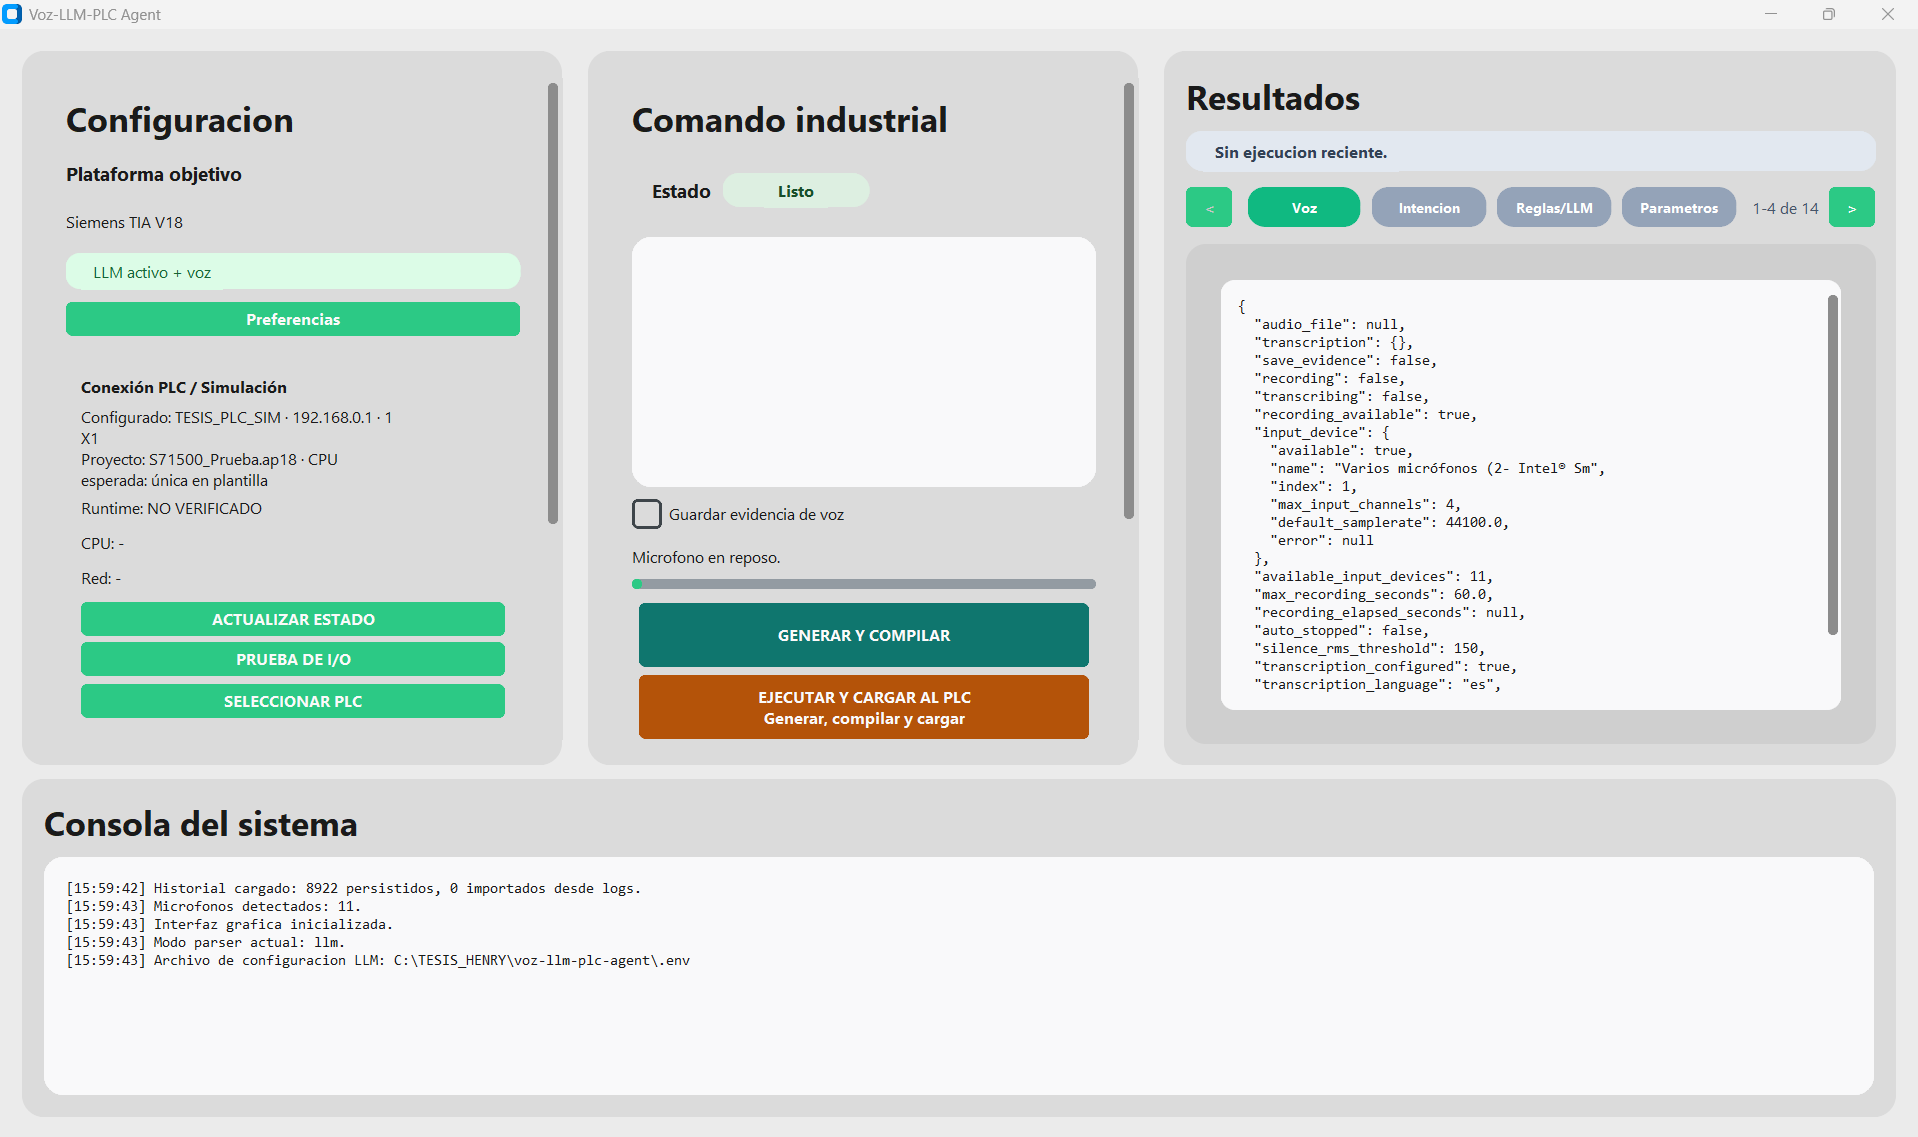
\includegraphics[width=.98\textwidth]{Graficos/Interfaz_Tesis.png}
\caption{Interfaz en su estado inicial: configuración, comando industrial, resultados y consola.}
\label{fig:interfaz_usuario}
\end{figure*}

\label{sec:semantica}
\label{sec:generacion}
El LLM actúa como intérprete semántico: identifica intención, requisitos, parámetros, señales y posibles aclaraciones. Conforme a la metodología aprobada, el LLM se integró con un motor local de generación basado en reglas, plantillas y estructuras IEC 61131-3: el modelo produce la interpretación y el motor la transforma en IR y SCL. Esta generación determinista delimita las composiciones admitidas y permite comprobar su estructura. El contexto incluye el mapa autorizado, el catálogo, reglas, ejemplos y documentación técnica recuperada localmente. El esquema valida campos, tipos y solicitudes de aclaración. Se empleó el identificador remoto \texttt{gpt-5.6-terra}, con espera de 45 s, hasta dos reintentos del envoltorio y respaldo semántico desactivado en la versión final. La solicitud no envía temperatura, semilla ni límite explícito de salida; el prompt y la configuración detallada se conservan en el archivo experimental del proyecto.

La IR conserva variables, tipos, direcciones, bloques, tarea e instancias; temporizadores, contadores y flancos mantienen estado en el FB. Las memorias internas se distinguen de los canales externos y los literales \texttt{T\#...} representan tiempos. El alcance de generación está delimitado por el catálogo y las composiciones implementadas.

\label{sec:verificacion}
El verificador comprueba estructura, declaraciones, tipos soportados, direcciones, recursos, instancias IEC y propagación de requisitos. Admite reparaciones e interpretaciones acotadas; un rechazo detiene las etapas dependientes y conserva el diagnóstico. El flujo interactivo permite responder aclaraciones y continuar.

\subsection{Mapa I/O y asignación de recursos}
\label{sec:mapa_io}
El mapa I/O delimita los recursos autorizados mediante dirección, tipo, clase, estado y permisos. El resolvedor vincula las funciones solicitadas con canales compatibles; una variable interna no sustituye una entrada o salida externa. Los canales \texttt{LOCKED} mantienen su asignación protegida, los \texttt{FREE} están disponibles y la reutilización de los \texttt{ASSIGNED} depende de su procedencia. En una ampliación se conserva el programa como contexto; al crear un programa nuevo pueden liberarse asignaciones automáticas, preservando las manuales, persistentes y bloqueadas.

Los 180 comandos utilizaron copias independientes de un mismo mapa de simulación: ocho entradas y ocho salidas digitales BOOL (Tabla~\ref{tab:mapa_io}). Tres entradas permanecieron protegidas: arranque, parada y condición lógica de emergencia. Las otras cinco entradas y las ocho salidas estaban disponibles al inicio de cada ensayo. La señal \texttt{I\_Emergency} se declaró explícitamente como recurso autorizado para el rol \texttt{SAFETY\_TRIP}; representa una condición lógica simulada. El mapa también declara cuatro entradas y cuatro salidas analógicas, que no intervinieron en esta evaluación.

Las asignaciones de un comando no se heredaron al siguiente. Cada registro conserva el mapa inicial, su huella y la instantánea de los recursos resueltos. El contexto del LLM contiene nombres, alias, estados y descripciones; los canales digitales disponibles tenían descripciones vacías y conservaron sus nombres y alias de inventario.
\begin{table*}[t]
\caption{Mapa digital común al inicio de cada ensayo. DI: entrada digital; DO: salida digital. La asignación efectiva de los canales disponibles se conserva por comando.}
\label{tab:mapa_io}
\centering\footnotesize
\begin{tabularx}{\textwidth}{@{}l l l l >{\raggedright\arraybackslash}X@{}}
\toprule Dirección & Símbolo protegido & Tipo & Clase & Estado inicial\\ \midrule
\texttt{\%I16.0} & \path{I_Start} & BOOL & DI & LOCKED; arranque\\
\texttt{\%I16.1} & \path{I_Stop} & BOOL & DI & LOCKED; parada\\
\texttt{\%I16.2} & \path{I_Emergency} & BOOL & DI & LOCKED; condición lógica de emergencia\\
\texttt{\%I16.3}--\texttt{\%I16.7} & --- & BOOL & DI & FREE; función asignable por ensayo\\
\texttt{\%Q8.0}--\texttt{\%Q8.7} & --- & BOOL & DO & FREE; función asignable por ensayo\\
\bottomrule
\end{tabularx}
\end{table*}

\subsection{Integración y banco de simulación}
\label{sec:integracion}
\label{sec:bancos}
TIA Openness importa fuente y tags, compila y registra errores y advertencias. El paquete contiene el FB \texttt{PLC\_PRG}, su DB de instancia y \texttt{Main} (OB1), que llama al FB. La descarga depende de la configuración y autorización del destino; compilación, descarga y RUN se registran por separado. En los ensayos se utilizó una copia nueva del maestro y se archivó el proyecto antes de descargar. La Figura~\ref{fig:integracion_tia_d01} ilustra la integración de una solicitud interactiva equivalente a D01.

\begin{figure*}[!tp]
\centering
\textbf{(a)}\par\smallskip
\includegraphics[width=.98\textwidth,trim=330bp 374bp 278bp 198bp,clip]{Graficos/D01_TIA.png}
\par\medskip
\textbf{(b)}\par\smallskip
\includegraphics[width=.98\textwidth,trim=210bp 80bp 278bp 426bp,clip]{Graficos/D01_TIA.png}
\caption{Ejemplo interactivo en TIA: (a) llamada al DB de instancia; (b) compilación con cero errores y advertencias. Recortes de presentación de la captura original.}
\label{fig:integracion_tia_d01}
\end{figure*}
\begin{table}[t]
\caption{Entorno de ingeniería y simulación.}
\label{tab:hardware}
\small
\begin{tabularx}{\linewidth}{@{}l >{\raggedright\arraybackslash}X@{}}
\toprule Elemento & Configuración\\ \midrule
Ingeniería & TIA Portal V18 y Openness\\
CPU objetivo & S7-1500 1516-3 PN/DP, firmware V2.6\\
Simulación & S7-PLCSIM Advanced V5\\
Aplicación & Python 3.13.15\\
\bottomrule
\end{tabularx}
\end{table}
El período conceptual de 100 ms de la IR es un metadato; OB1 utiliza su configuración efectiva. Se utilizó la instancia virtual \texttt{TESIS\_PLC\_SIM}, con dirección \texttt{192.168.0.1} y comunicación TCP/IP.


\subsection{Corpus y reconocimiento de voz}
\label{sec:asr}
El corpus contiene 60 locuciones humanas de un participante S01 y 60 derivados ruidosos pareados, en WAV PCM16, mono y 16 kHz. La captura usa \texttt{sounddevice}; el ASR remoto \texttt{gpt-4o-mini-transcribe} recibe español, respuesta JSON y temperatura 0, con espera de 30 s y un reintento por conexión o tiempo de espera. El prompt aporta vocabulario industrial general y cada ejecución conserva modelo, solicitud y transcripción original. La elección del ASR respondió a un criterio práctico de costo y al propósito exploratorio de comprobar la viabilidad del flujo con una opción económica. No se realizó una comparación previa de WER o latencia entre modelos ASR alternativos. Los WER obtenidos en la campaña final (4,79\,\% en voz limpia y 6,91\,\% con ruido), considerados junto con los resultados de ejecución, respaldan a posteriori la viabilidad de esta opción para el catálogo evaluado.

La transcripción se entrega al LLM sin reescritura lingüística previa, salvo eliminar espacios en los extremos. La interpretación del vocabulario técnico y la desambiguación corresponden al módulo semántico, que puede solicitar aclaraciones. La normalización para calcular el WER se aplica únicamente a la evaluación y no sustituye la transcripción enviada al intérprete.

La condición ruidosa utiliza SNR de $10\pm0{,}25$ dB. Cada derivado conserva la locución de origen y se obtiene mediante
\begin{equation}
y=x+\alpha n,\qquad \alpha=\sqrt{\frac{P_x}{P_n10^{10/10}}},
\end{equation}
donde $x$ es la voz limpia, $n$ el ruido y $P_x$ y $P_n$ sus potencias medidas. El ruido maestro procedía de un archivo ambiental de Pixabay convertido al formato canónico. Las potencias se midieron entre la primera y la última trama activa de voz: tramas de 20 ms, umbral relativo de $-30$ dB respecto del máximo RMS y mínimo de 50 unidades PCM16. Cada caso--variante recibió un segmento determinista del mismo ruido maestro. Tras cuantificar la mezcla se verificaron la ausencia de saturación y el SNR dentro de la tolerancia declarada. Los parámetros de mezcla y los manifiestos se conservan en el archivo experimental del proyecto.

\subsection{Casos y diseño experimental}
\label{sec:casos}
\label{sec:condiciones}
Se evaluó la versión final mediante veinte requisitos discretos del catálogo del proyecto, con tres variantes lingüísticas por caso: tres casos de complejidad baja, diez media y siete alta (Apéndice~\ref{app:casos}). La unidad experimental es cada comando caso--variante--modalidad; los lotes automatizan su ejecución y archivo. El diseño comprende $20\times3\times3=180$ celdas, ejecutadas en el orden texto, voz limpia y voz con ruido. Las dos condiciones acústicas comparten la locución de origen.

La configuración empleó exclusivamente interpretación LLM, con el respaldo por reglas desactivado. Se seleccionó un resultado por celda, independientemente de su veredicto. Las aclaraciones finalizaron sin respuesta del usuario. Los errores técnicos admitían hasta dos reintentos automáticos con esperas de 5 y 15 s y conservación del intento y su motivo; los fallos de interpretación funcional, asignación, compilación o comportamiento no autorizaban repetir hasta obtener éxito. Durante la ejecución se rectificó una clasificación: D14--V3 textual pasó de \texttt{INFRASTRUCTURE\_ERROR} a FAIL por un rechazo de asignación I/O. La clasificación inicial había originado un reintento improcedente con PASS, que se conservó pero se excluyó del análisis. Hubo, por tanto, un único reintento total y ninguno por una incidencia técnica real. La auditoría conserva el registro original y la justificación de la rectificación.

El motor de interpretación y generación, el prompt, el mapa, las plantillas de prueba y los archivos de audio se identificaron mediante huellas antes de ejecutar la campaña. Cada comando utilizó un proyecto aislado y conservó los artefactos disponibles de sus etapas. El Apéndice~\ref{app:reproducibilidad} identifica la campaña y su documentación reproducible.

Una campaña preliminar con la misma matriz identificó el respaldo por reglas activo y un mapa distinto del previsto en D05. Para la evaluación final se fijaron la interpretación LLM exclusiva y el mapa común y se ejecutaron nuevamente los 180 comandos, conservando el prompt, el reconocimiento de voz, los Oracles y los archivos de audio. Los resultados principales corresponden a esta campaña final; los registros preliminares permanecen en el archivo experimental. Las versiones de código y configuración se identifican por separado: no se presupone identidad del generador entre campañas.

\subsection{Oracles y conformidad experimental}
\label{sec:oracles}
Cada Oracle es una plantilla JSON con roles, precondiciones, estímulos, respuestas, ventanas temporales, invariantes y restauración. Se elaboró con asistencia de IA a partir del requisito. Las tres variantes y modalidades de un caso comparten la misma plantilla, fijada antes de la campaña; sus expectativas permanecen fuera del contexto del generador.

El ejecutor aplica entradas, adquiere salidas y compara las trazas (Figura~\ref{fig:bancos}). Para el caso $j$, la conformidad experimental requiere verificación local, compilación TIA y aceptación global del Oracle:
\begin{equation}
A_j(P)=V_{\mathrm{local}}(P,M)\land C_{\mathrm{TIA}}(P)
\land[O_j(P)=\mathrm{PASS}].
\label{eq:aceptable}
\end{equation}
Aquí $M$ es el mapa autorizado y $P$ el programa. El veredicto $O_j$ combina la correspondencia semántica exigida, la resolución de roles y las comprobaciones funcionales, temporales e invariantes sobre la traza, bajo los estímulos y el horizonte del caso. Un estado de salida correcto no basta cuando falta un rol o existe una discrepancia semántica pendiente de resolver.
\begin{figure*}[!tp]
\centering
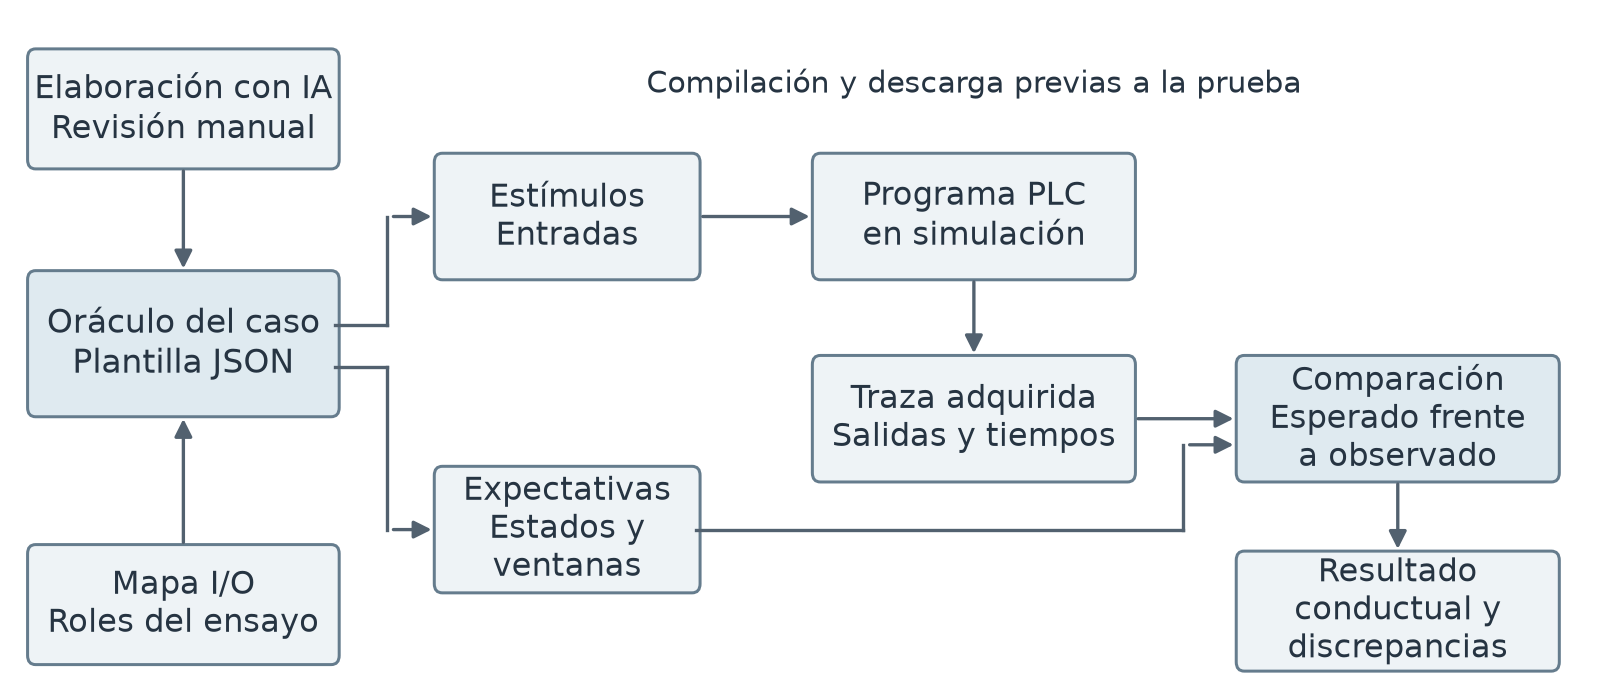
\includegraphics[width=\textwidth]{Graficos/oracle_evaluacion_discreta.png}
\caption{Evaluación experimental: estímulos definidos por el Oracle, adquisición de trazas y contraste con expectativas separadas del generador.}
\label{fig:bancos}
\end{figure*}
Las señales de prueba son activas en TRUE; en D15, \texttt{MODE\_AUTO=TRUE} selecciona Automático y FALSE, Manual. Se solicitó adquisición cada 50 ms con reloj monótono. Las plantillas fijadas antes de la campaña establecen las tolerancias como convenciones experimentales: D01 y D17 admiten 4,7--5,7 s alrededor del nominal de 5 s, equivalentes a márgenes de $-300$ y $+700$ ms; D07 exige arranque retardado, con comprobaciones antes y después de 3 s. En D05, la comprobación del invariante excluye las muestras de los 100 ms posteriores a cada escritura de entradas como margen de propagación. Estos márgenes son criterios de aceptación del protocolo y no estimaciones de precisión del PLC. Las marcas reales de adquisición delimitan el tiempo observado y no identifican las transiciones con precisión de un ciclo PLC. Por ejemplo, D01 parte de entrada y salida desactivadas, aplica un pulso de arranque de 300 ms y comprueba que la salida se active, permanezca encendida al liberar el pulsador y se apague dentro de la ventana declarada. Las secuencias completas, los estados iniciales y las tolerancias por caso se conservan en el archivo experimental del proyecto.

\subsection{Métricas y análisis estadístico}
\label{sec:metricas}
\label{sec:estadistica}
Se informan estados por etapa, compilación, conformidad y cobertura del evaluador. La correspondencia semántica compuesta reúne comprobaciones evaluables de intención, roles y parámetros; por ejemplo, en D05 contrasta la prioridad de emergencia y los roles de arranque, disparo y motor. La aceptación del esquema semántico se distingue de esta correspondencia con el requisito. Las tasas describen el resultado final de cada unidad experimental dentro del flujo implementado, incluidas las normalizaciones, reparaciones y reinterpretaciones internas permitidas. No se calculó una tasa independiente de acierto de la primera respuesta del LLM.

En voz, la tasa de error de palabras (WER, por sus siglas en inglés) cuantifica la discrepancia entre la transcripción y el texto de la variante que el participante debía leer. Se alinean ambas secuencias mediante distancia de Levenshtein por palabras, buscando el número mínimo de operaciones de edición:
\begin{equation}
\mathrm{WER}=\frac{S+D+I}{N_{\mathrm{palabras}}},
\label{eq:wer}
\end{equation}
donde $S$ cuenta las sustituciones de palabras, $D$ las palabras omitidas, $I$ las palabras añadidas y $N_{\mathrm{palabras}}$ las palabras de referencia. El resultado se expresa como porcentaje: una sustitución en una referencia de diez palabras equivale a 10\,\%. La normalización aplica Unicode NFC, \texttt{casefold}, sustitución de caracteres no alfanuméricos por espacios y colapso de espacios; conserva tildes y distingue palabras numéricas de dígitos, como ``cinco'' y ``5''. El WER global se obtiene sumando los errores de las 60 transcripciones y dividiendo por el total de palabras de referencia; no se promedian sus tasas individuales. Esta métrica describe coincidencia textual, mientras que la conservación del requisito se contrasta mediante la evaluación semántica y el Oracle.

Las duraciones se resumen con media, desviación estándar muestral, mediana y cuartiles inclusivos; los campos ausentes no se imputan. El total registrado incluye la instrumentación del ensayo, excluye captura previa y pausas entre comandos. Los hitos acumulados de semántica y generación no se suman como etapas independientes.

Se calculó Wilson al 95\,\% como referencia binomial orientativa \citep{nistWilson}. Las diferencias de conformidad entre modalidades se estimaron mediante bootstrap exploratorio por caso para conservar la dependencia \citep{field2007bootstrapcluster}: veinte casos remuestreados con reposición, sus tres variantes juntas e índices compartidos entre modalidades; 20\,000 réplicas, semilla 20261026 y percentiles 2,5/97,5. El indicador pareado acredita exclusivamente PASS. Los scripts de cálculo y el contraste independiente de transcripciones, asignaciones y conteos se conservan en el archivo experimental del proyecto.
Como análisis complementario, se compararon los veredictos PASS, FAIL y REVIEW de las mismas 180 celdas entre la campaña preliminar y la final. Se calcularon el acuerdo exacto y el kappa no ponderado de Cohen, $\kappa=(p_o-p_e)/(1-p_e)$, donde $p_o$ es la proporción de coincidencias y $p_e$ el acuerdo esperado a partir de las frecuencias marginales. Esta comparación no se incorpora a las tasas de la campaña final.
\ifdefined\FloatBarrier\FloatBarrier\fi


\section{\TituloResultados}
\label{sec:resultados}
La campaña final completó las 180 celdas previstas, sin ausencias ni duplicados: 165 PASS, siete FAIL y ocho REVIEW. La Tabla~\ref{tab:resultados_modalidad} resume los resultados por modalidad. Las tres obtuvieron la misma conformidad global, aunque difirieron los comandos aceptados y la etapa de detención.
\begin{table*}[t]
\caption{Resultados de la versión final. El IC Wilson al 95\,\% es una referencia descriptiva; la comparación pareada se presenta en la Tabla~\ref{tab:pareadas}.}
\label{tab:resultados_modalidad}
\small
\begin{tabularx}{\textwidth}{@{}X r r r r r l@{}}
\toprule Modalidad & Compilan & PASS & FAIL & REVIEW & Conformidad & IC Wilson (\%)\\ \midrule
Texto & 58/60 & 55 & 3 & 2 & 91,67\,\% & 81,93--96,39\\
Voz limpia & 59/60 & 55 & 1 & 4 & 91,67\,\% & 81,93--96,39\\
Voz con ruido & 57/60 & 55 & 3 & 2 & 91,67\,\% & 81,93--96,39\\
\bottomrule
\end{tabularx}
\end{table*}

\subsection{Generación e integración}
Se construyeron y verificaron localmente 176 paquetes: 59 de texto, 59 de voz limpia y 58 con ruido. Compilaron 174 y todos se descargaron y acreditaron conexión en RUN (Tabla~\ref{tab:etapas_modalidades}). Las cuatro detenciones previas a la generación correspondieron a una asignación I/O rechazada y tres solicitudes de aclaración. El contraste independiente verificó 755 señales digitales vinculadas, sin reasignación de las tres entradas protegidas ni incompatibilidad de tipo o clase en los canales resueltos.
\begin{table}[t]
\caption{Aceptaciones por etapa. T: texto; L: voz limpia; R: voz con ruido. Los veredictos globales se distinguen de las comprobaciones funcionales aisladas.}
\label{tab:etapas_modalidades}
\small
\begin{tabularx}{\linewidth}{@{}X r r r@{}}
\toprule Etapa & T & L & R\\ \midrule
IR y verificación local & 59 & 59 & 58\\
Compilación TIA & 58 & 59 & 57\\
Descarga & 58 & 59 & 57\\
Conexión RUN & 58 & 59 & 57\\
Aceptación global & 55 & 55 & 55\\
\bottomrule
\end{tabularx}
\end{table}

\subsection{Reconocimiento y comparación pareada}
Las 60 parejas conservaron la locución de origen y cumplieron el formato y la tolerancia de SNR. Con 1085 palabras de referencia por condición, el WER global fue 4,79\,\% en voz limpia y 6,91\,\% con ruido: un aumento observado de 2,12 puntos porcentuales (Tabla~\ref{tab:wer_modalidades} y Figura~\ref{fig:wer_pareado}).
\begin{table}[t]
\caption{Errores de reconocimiento agregados. S/D/I: sustituciones, eliminaciones e inserciones; $N$: palabras de referencia.}
\label{tab:wer_modalidades}
\small
\begin{tabularx}{\linewidth}{@{}X r r r r r@{}}
\toprule Condición & S & D & I & $N$ & WER\\ \midrule
Limpia & 43 & 4 & 5 & 1085 & 4,79\,\%\\
Ruido & 63 & 0 & 12 & 1085 & 6,91\,\%\\
\bottomrule
\end{tabularx}
\end{table}
\begin{figure*}[!tp]
\centering
\includegraphics[width=.94\textwidth]{Graficos/wer_pareado.png}
\caption{WER de las 60 parejas caso--variante. Los círculos representan voz limpia y las cruces, ruido; cada segmento vertical enlaza la misma locución. Las tasas globales se calculan mediante errores y palabras agregados.}
\label{fig:wer_pareado}
\end{figure*}
Las diferencias pareadas de conformidad fueron cero en las tres comparaciones, con intervalos que incluyen valores positivos y negativos (Tabla~\ref{tab:pareadas}). Entre voz limpia y ruido hubo 53 parejas con PASS en ambas condiciones y dos con PASS exclusivo de cada una. La coincidencia de las tasas no implica identidad de resultados por comando.
\begin{table*}[t]
\caption{Conformidad pareada: diferencia B menos A e IC exploratorio por caso al 95\,\%, en puntos porcentuales. Ninguna: pareja sin PASS en las dos condiciones.}
\label{tab:pareadas}
\small
\begin{tabularx}{\textwidth}{@{}X r r r r r l@{}}
\toprule A $\rightarrow$ B & Ambas & Solo A & Solo B & Ninguna & Diferencia & IC por caso\\ \midrule
Texto $\rightarrow$ limpia & 52 & 3 & 3 & 2 & $0,00$ & $[-10,00;\ 8,33]$\\
Texto $\rightarrow$ ruido & 52 & 3 & 3 & 2 & $0,00$ & $[-6,67;\ 6,67]$\\
Limpia $\rightarrow$ ruido & 53 & 2 & 2 & 3 & $0,00$ & $[-5,00;\ 5,00]$\\
\bottomrule
\end{tabularx}
\end{table*}

\subsection{Complejidad y duración}
Todos los casos de complejidad baja obtuvieron PASS. En los grupos medio y alto aparecieron fallos y revisiones (Tabla~\ref{tab:complejidad}). Quince casos de texto, diecisiete de voz limpia y dieciséis con ruido obtuvieron PASS en sus tres variantes. La agrupación es descriptiva y no aísla el efecto de la complejidad frente al contenido del requisito.
\begin{table}[t]
\caption{Resultados por complejidad: compilados / conformes. Baja: $n=9$; media: $n=30$; alta: $n=21$.}
\label{tab:complejidad}
\small
\begin{tabularx}{\linewidth}{@{}>{\raggedright\arraybackslash}X r r r@{}}
\toprule Modalidad & Baja & Media & Alta\\ \midrule
Texto & 9 / 9 & 30 / 28 & 19 / 18\\
Voz limpia & 9 / 9 & 29 / 29 & 21 / 17\\
Voz con ruido & 9 / 9 & 29 / 29 & 19 / 17\\
\bottomrule
\end{tabularx}
\end{table}
La duración media registrada fue 55,19 s en texto, 52,23 s en voz limpia y 52,78 s con ruido (Tabla~\ref{tab:latencias}). La operación TIA tuvo medias de 40,56, 37,29 y 37,05 s, respectivamente, lo que contribuye a la diferencia observada en el total. El orden fijo y la composición de las etapas ejecutadas impiden atribuir esa diferencia a una ventaja causal de la voz.
\begin{table*}[t]
\caption{Duración registrada del ensayo automatizado, en segundos. DE: desviación estándar; Q1 y Q3: cuartiles inclusivos. $n$ cuenta los registros con este campo disponible.}
\label{tab:latencias}
\small
\begin{tabularx}{\textwidth}{@{}X r r r r r@{}}
\toprule Modalidad & $n$ & Media $\pm$ DE & Mediana & Q1 & Q3\\ \midrule
Texto & 59 & $55,19\pm9,94$ & 53,17 & 49,84 & 56,92\\
Voz limpia & 59 & $52,23\pm5,87$ & 50,34 & 48,52 & 54,51\\
Voz con ruido & 58 & $52,78\pm7,20$ & 50,50 & 48,53 & 55,17\\
\bottomrule
\end{tabularx}
\end{table*}

\subsection{Trazas y resultados sin conformidad acreditada}
D05--V1 obtuvo PASS en las tres modalidades. Los roles de arranque, emergencia y motor utilizaron las direcciones \texttt{\%I16.0}, \texttt{\%I16.2} y \texttt{\%Q8.4}, respectivamente. La Figura~\ref{fig:d05_modalidades} presenta las 70 muestras por modalidad. La primera muestra del motor apagado se adquirió unos 50--65 ms después de la primera muestra de emergencia activa. Este intervalo observado incluye ejecución y adquisición; el PASS corresponde a las comprobaciones y ventanas del Oracle.
\begin{figure*}[!tp]
\centering
\includegraphics[width=.94\textwidth]{Graficos/d05_tres_modalidades.png}
\caption{D05--V1 en las tres modalidades. Señales BOOL desplazadas verticalmente: cada una presenta 0 abajo y 1 arriba. Puntos: muestras; segmentos: último valor observado. El tiempo parte del inicio de cada evaluación. Al cambiar la emergencia aparecen muestras transitorias antes de observar la respuesta del motor; la traza no mide un tiempo de reacción con precisión de ciclo PLC.}
\label{fig:d05_modalidades}
\end{figure*}

En D07--V2 textual, el programa compiló pero produjo un pulso inmediato de unos 3 s en lugar del arranque retardado solicitado. La primera muestra ON apareció 0,066 s después del inicio del paso de arranque (Figura~\ref{fig:respuesta_discreta}), incumpliendo las comprobaciones de salida apagada antes de 2,7 s. Esta discrepancia muestra por qué la compilación no acredita el cumplimiento del requisito.
\begin{figure*}[!tp]
\centering
\includegraphics[width=.94\textwidth]{Graficos/d07_traza_texto.png}
\caption{D07--V2 textual: entrada de arranque y salida del motor medidas, referidas al inicio del paso de prueba. La línea de 3 s es la referencia nominal de arranque; antes de 2,7 s el Oracle exige salida apagada. Los puntos muestran adquisición y los segmentos mantienen el último valor observado.}
\label{fig:respuesta_discreta}
\end{figure*}

La Tabla~\ref{tab:errores} separa los siete fallos confirmados de los ocho REVIEW. Los fallos fueron tres aclaraciones, una asignación rechazada, dos rechazos de compilación por tipos y la discrepancia conductual de D07. Las aclaraciones correspondieron a D05--V2 en ambas condiciones acústicas y D17--V3 con ruido. Solicitar información cumple RF3; se contabilizó como fallo de resolución autónoma porque el protocolo no respondía y el ensayo terminó sin programa ejecutable.
\begin{table}[t]
\caption{Etapa terminal de los resultados sin conformidad acreditada. T: texto; L: voz limpia; R: voz con ruido.}
\label{tab:errores}
\small
\begin{tabularx}{\linewidth}{@{}>{\raggedright\arraybackslash}X r r r@{}}
\toprule Etapa o estado & T & L & R\\ \midrule
Semántica: aclaración & 0 & 1 & 2\\
Asignación I/O & 1 & 0 & 0\\
Compilación TIA & 1 & 0 & 1\\
Discrepancia conductual & 1 & 0 & 0\\ \midrule
Subtotal FAIL & 3 & 1 & 3\\
REVIEW & 2 & 4 & 2\\
\bottomrule
\end{tabularx}
\end{table}

Siete REVIEW no resolvieron todos los roles exigidos: D15--V3 en texto; D15--V2/V3 y D17--V1/V3 en voz limpia; D15--V1/V3 con ruido. El restante, D05--V2 textual, superó las comprobaciones funcionales pero presentó discrepancia entre su intención semántica y la exigida por el Oracle. Por ello, la aceptación global y el resultado funcional aislado no son intercambiables. Los diagnósticos y las expectativas incumplidas se conservan por comando.

De los 174 informes de ejecución, 49 evaluaron invariantes explícitos sin registrar violaciones críticas o mayores; 118 correspondieron a casos sin esos invariantes y siete no completaron su evaluación por falta de roles. Estas cifras describen la cobertura del evaluador.


\section{\TituloDiscusion}
\label{sec:discusion}
\subsection{Conservación del requisito y efecto de la entrada}
La arquitectura acreditó conformidad en 165 de 180 comandos. La diferencia entre 174 compilaciones aceptadas y 165 PASS muestra la aportación de comprobar semántica, roles y comportamiento además de sintaxis. El aumento de WER de 4,79\,\% a 6,91\,\% coexistió con la misma tasa global de conformidad en las tres modalidades. Sin embargo, las parejas discordantes y los intervalos de las diferencias no permiten establecer equivalencia ni superioridad.

El LLM interpreta el requisito; la IR y el SCL se construyen mediante plantillas y reglas locales. El desempeño observado corresponde a esa cadena completa de interpretación y composición. La separación facilita revisar cómo una discrepancia semántica se transforma en código ejecutable, como ocurrió con el pulso de D07.

La propuesta comparte con LLM4PLC la interacción y las comprobaciones externas, aunque aquí se evalúan trazas de horizonte finito en lugar de SMV \citep{fakih2024llm4plc}. SemaPLC también integra contexto y comportamiento \citep{tu2026semaplc}; este trabajo articula esos elementos mediante un mapa autorizado, IR e integración Siemens. La complementariedad de comprobaciones \citep{schnakenbeck2026comparison} y la relación entre estímulos y cobertura \citep{ma2019plantfeatures} condicionan cualquier comparación de tasas entre estudios.

\subsection{Propagación de discrepancias}
Los fallos se distribuyeron entre interpretación, asignación, tipado y comportamiento. En D14--V3 textual se rechazó una propuesta de asignación incompatible con los recursos; en D20--V1 textual y D20--V3 con ruido, TIA detectó incompatibilidades de tipos después de la verificación local. D07--V2 textual superó la compilación pero confundió duración de pulso y retardo de arranque. Estas observaciones justifican conservar los artefactos intermedios y los diagnósticos de cada etapa.

% Cita literal contrastada con los dos audio/asr_result.json de D05--V2: comienza con "lo apague", no con "no apague".
Las transcripciones de D05--V2 en ambas condiciones acústicas incluyeron \guillemotleft{}lo apague y lo deje arrancado mientras dure\guillemotright{}, y el intérprete pidió aclaración. Frente a la restricción prevista \guillemotleft{}no deje arrancarlo\guillemotright{}, la transcripción \guillemotleft{}lo deje arrancado\guillemotright{} invierte el sentido de la negación y contradice el bloqueo del arranque durante la emergencia. Sin contrastar la lectura real con el audio no puede atribuirse toda esa contradicción al ASR: WER compara con el texto previsto. En D17--V3 con ruido, la aclaración distinguió ausencia de detección y ausencia de cambios del sensor. Los REVIEW por roles ausentes muestran, además, que disponer de código compilable no garantiza compatibilidad entre la interpretación obtenida y el contrato de prueba.

Los REVIEW presentaron causas diferentes. En D15 se observaron diferencias entre la representación del selector Manual/Automático y los roles requeridos por el evaluador. En D17 faltó el rol \texttt{START} y, en el programa inspeccionado, también se omitió la condición de habilitación mediante arranque. En D05--V2 textual, las comprobaciones funcionales fueron satisfactorias, pero la etiqueta de intención no coincidió con la admitida por el Oracle. Estos casos requieren revisar la correspondencia entre requisito, interpretación y programa antes de determinar si procede corregir la generación, el enlace de roles o el criterio de evaluación. Los veredictos originales se conservaron.

\subsection{Alcance y limitaciones}
Los casos D01--D20 pertenecen al catálogo que el generador implementa; los resultados no describen el desempeño ante requisitos fuera de ese catálogo. Se evaluaron tres variantes por caso, un locutor y una configuración Siemens simulada. S01 fue el primer autor y desarrollador del sistema. La ejecución única por celda y el orden fijo limitan la estimación de variabilidad y la atribución causal de diferencias entre modalidades. Los intervalos por caso son exploratorios; los intervalos Wilson no incorporan la dependencia entre variantes. El servicio remoto se identifica por su nombre de modelo, sin instantánea inmutable acreditada, semilla ni temperatura explícita en la solicitud LLM. Esta evaluación no incluyó un grupo de programación manual ni una comparación con la generación local sin LLM. Por tanto, sus resultados caracterizan la arquitectura completa y no cuantifican mejoras de productividad ni la contribución aislada de cada componente.

Las tasas principales conservan las 60 celdas previstas por modalidad. REVIEW señala una decisión global no acreditada, por roles ausentes o discrepancia semántica, y se mantiene separado de PASS y FAIL. Los Oracles tuvieron validación de contenido mediante revisión manual del investigador, con asistencia de IA en su elaboración y expectativas separadas del generador. No se realizó un contraste independiente en PLCSIM con programas de referencia revisados por otro especialista; sus estímulos, tolerancias y cobertura limitan la fuerza de la evaluación. La adquisición solicitada cada 50 ms y las ventanas de respuesta no acreditan ausencia de transitorios de menor duración ni certifican seguridad industrial.

Entre las campañas preliminar y final coincidieron 157 de los 180 veredictos (87,22\,\%; $\kappa=0,253$), considerando PASS, FAIL y REVIEW como categorías distintas. La elevada frecuencia de PASS influye en el valor de kappa; además, solo seis celdas quedaron sin conformidad acreditada en ambas campañas, por lo que los fallos individuales se interpretan como observaciones de cada ejecución y versión, sin asumir que sean propiedades estables de cada comando. Es una comparación indicativa entre versiones, no una estimación de repetibilidad con configuración idéntica, porque cambiaron las condiciones de asignación, respaldo y código. Con los mismos 60 audios limpios, el WER global pasó de 4,88\,\% a 4,79\,\% por una sustitución menos en D10--V1; esta variación observada entre invocaciones tampoco permite suponer una transcripción remota invariable.

\subsection{Implicaciones prácticas y trabajo futuro}
La trazabilidad facilita revisar el paso de la instrucción a las señales, el código y la respuesta observada, y localizar las etapas que requieren intervención. El trabajo futuro evaluará más locutores, ruido industrial real y comandos fuera del catálogo, comparará modelos ASR alternativos, incluidos modelos locales, y contrastará los Oracles con programas de referencia independientes y mediciones temporales de mayor resolución.


\section{\TituloConclusiones}
\label{sec:conclusiones}
Se desarrolló una arquitectura voz/texto--LLM--PLC que interpreta requisitos mediante el LLM y construye localmente IR y SCL, con integración Siemens. La versión final se evaluó con 180 comandos, un mapa I/O común y expectativas separadas del generador. Compilaron 174 programas y 165 obtuvieron PASS: 55/60 (91,67\,\%) en cada modalidad. Los siete fallos y ocho REVIEW identificaron discrepancias de interpretación, asignación, tipos, roles y comportamiento.

El WER global fue 4,79\,\% en voz limpia y 6,91\,\% con ruido. La diferencia de conformidad ruido menos limpia fue 0,00 puntos porcentuales, con IC exploratorio por caso $[-5,00;\ 5,00]$. La igualdad de las tasas no demuestra equivalencia entre modalidades. Los resultados sustentan la viabilidad de la cadena para el catálogo discreto evaluado en simulación y muestran la necesidad de comprobar el programa más allá de su compilación.
\ifdefined\FloatBarrier\FloatBarrier\fi


\section*{Contribuciones de autoría CRediT}
% CONFIRMAR: revisar los roles CRediT propuestos antes de la versión final.
Henry Fernando Ochoa Zea: Conceptualización, Metodología, Software, Investigación, Análisis formal, Curación de datos, Visualización, Redacción -- borrador original.\par
% CONFIRMAR: revisar los roles CRediT propuestos del tutor antes de la versión final.
Paul Andres Chasi Pesantez: Supervisión, Validación, Redacción -- revisión y edición.\par
\section*{Declaración de conflictos de interés}
Los autores declaran no tener conflictos de interés.
\section*{Financiamiento}
Esta investigación no recibió financiamiento específico de agencias públicas, comerciales ni sin fines de lucro.
% Declaración de disponibilidad de datos omitida en esta versión para la maestría.

\section*{Declaración sobre el uso de inteligencia artificial generativa}
Durante la preparación de este manuscrito se utilizaron ChatGPT y Codex (OpenAI) para apoyar la redacción y reorganización de secciones, mejorar la claridad y coherencia del texto, consultar y contrastar información bibliográfica y revisar la correspondencia de la descripción metodológica con el código y los registros del proyecto. También se emplearon para editar el código LaTeX y elaborar figuras a partir de los datos experimentales registrados. La responsabilidad por el contenido, la exactitud de las referencias y la interpretación de los resultados corresponde a los autores.
\section*{Agradecimientos}
El primer autor agradece a su familia el apoyo constante, la comprensión y el acompañamiento en cada etapa de su formación y en el desarrollo de este trabajo.

% Referencias seleccionadas y fuentes de contraste documentadas en referencias.bib.


\FloatBarrier
\bibliographystyle{cas-model2-names}
\bibliography{referencias}

\appendix
\section{Lista de casos de prueba}
\label{app:casos}
La Tabla~\ref{tab:catalogo_completo} presenta los casos D01--D20 y sus roles de entrada y salida. La asignación de cada rol a símbolos y direcciones se conserva en el mapa del ensayo. La Tabla~\ref{tab:variantes_textuales} reproduce las 60 variantes textuales, agrupadas por caso. El prompt completo y los mapas JSON se conservan en el archivo experimental del proyecto.

\begin{table*}[tp]
\caption{Catálogo discreto y roles requeridos. Cada caso aporta nueve celdas evaluadas: tres variantes en tres modalidades.}
\label{tab:catalogo_completo}
\footnotesize
\begin{tabularx}{\textwidth}{@{}l >{\raggedright\arraybackslash}X l >{\raggedright\arraybackslash}X >{\raggedright\arraybackslash}X@{}}
\toprule Caso & Requisito resumido & Complejidad & Roles de entrada & Roles de salida\\ \midrule
D01 & Salida temporizada de 5 s & Baja & \path{START} & \path{AUX_OUTPUT}\\
D02 & Lámpara mientras la entrada esté activa & Baja & \path{SENSOR} & \path{LAMP}\\
D03 & Arranque y paro con memoria de marcha & Baja & \path{START}, \path{STOP} & \path{MOTOR_MAIN}\\
D04 & Motor enclavado con Start y Stop & Media & \path{START}, \path{STOP} & \path{MOTOR_MAIN}\\
D05 & Prioridad de la condición de emergencia sobre el arranque & Media & \path{START_REQUEST}, \path{SAFETY_TRIP} & \path{MOTOR_MAIN}\\
D06 & Alarma por arranque sin condición de seguridad & Media & \path{START_REQUEST}, \path{SAFETY_OK} & \path{ALARM}\\
D07 & Arranque retardado 3 s con Start mantenido & Media & \path{START} & \path{MOTOR_MAIN}\\
D08 & Paro automático tras 10 s de funcionamiento continuo & Media & \path{START} & \path{MOTOR_MAIN}\\
D09 & Contador de 5 pulsos & Media & \path{PULSE_INPUT} & \path{COUNT_OUTPUT}\\
D10 & Contador de 5 pulsos con Reset & Media & \path{PULSE_INPUT}, \path{RESET} & \path{COUNT_OUTPUT}\\
D11 & Contactor con enclavamiento de marcha & Alta & \path{START}, \path{STOP} & \path{CONTACTOR}\\
D12 & Dos contactores con órdenes independientes e interbloqueo & Alta & \path{REQUEST_A}, \path{REQUEST_B} & \path{CONTACTOR_A}, \path{CONTACTOR_B}\\
D13 & Variador habilitado solo sin alarma & Media & \path{RUN_REQUEST}, \path{ALARM_ACTIVE} & \path{VFD_ENABLE}\\
D14 & Selección de velocidad baja/media/alta & Alta & \path{SPEED_LOW_CMD}, \path{SPEED_MEDIUM_CMD}, \path{SPEED_HIGH_CMD} & \path{SPEED_LOW}, \path{SPEED_MEDIUM}, \path{SPEED_HIGH}\\
D15 & Modo Manual/Automático con orden por modo & Alta & \path{MODE_AUTO}, \path{MANUAL_COMMAND}, \path{AUTO_COMMAND} & \path{MOTOR_MAIN}\\
D16 & Secuencia: principal, espera 3 s, auxiliar & Alta & \path{START} & \path{MAIN_OUTPUT}, \path{AUX_OUTPUT}\\
D17 & Supervisión de sensor 5 s tras Start & Alta & \path{START}, \path{SENSOR} & \path{ALARM}\\
D18 & Bloqueo del arranque en mantenimiento & Media & \path{MAINTENANCE}, \path{START} & \path{MOTOR_MAIN}\\
D19 & Pilotos de estado: detenido, marcha y falla & Media & \path{RUN_STATE}, \path{FAULT_ACTIVE} & \path{PILOT_STOPPED}, \path{PILOT_RUN}, \path{PILOT_FAULT}\\
D20 & Ciclo automático de 3 s con Reset & Alta & \path{START}, \path{RESET} & \path{RUN_OUTPUT}, \path{COMPLETE_STATE}\\
\bottomrule
\end{tabularx}
\end{table*}


% Una tabla lógica de variantes, distribuida en dos partes para conservar legibilidad.
\onecolumn
\begin{table*}[!ht]
\centering
\footnotesize
\setlength{\tabcolsep}{4pt}
\renewcommand{\arraystretch}{1.10}
\caption{Variantes textuales del catálogo discreto: D01--D10. Cada fila conserva las tres formulaciones evaluadas del mismo requisito.}
\label{tab:variantes_textuales}
\begin{tabularx}{\textwidth}{@{}l >{\raggedright\arraybackslash}X >{\raggedright\arraybackslash}X >{\raggedright\arraybackslash}X@{}}
\toprule Caso & V1 & V2 & V3\\ \midrule
D01 & Al presionar el pulsador, activa la salida digital durante 5 segundos. & Cuando se presione el pulsador, quiero que la salida se encienda durante cinco segundos. & Genera un pulso de salida de 5 segundos cada vez que se presione el pulsador.\\
\addlinespace[2pt]
D02 & Enciende la lámpara mientras la entrada digital esté activa. & Quiero que la lámpara esté encendida solo mientras la entrada esté activa. & Haz que la lámpara se encienda con la entrada digital activa y se apague cuando se desactive.\\
\addlinespace[2pt]
D03 & Arranca el motor con Start, mantenlo en marcha al soltar el pulsador y detenlo con Stop. & Quiero encender el motor con Start y que siga encendido aunque suelte el botón; con Stop se apaga. & Con memoria de marcha: Start enciende el motor, que permanece encendido al soltar el pulsador, y Stop lo apaga.\\
\addlinespace[2pt]
D04 & Enclava el motor con Start para que siga encendido al soltar el pulsador y apágalo con Stop. & Haz un enclavamiento: el motor arranca con Start, se queda encendido aunque se suelte el botón y se apaga con Stop. & Con Stop se apaga el motor; con Start se enciende y queda enclavado aunque se suelte el pulsador.\\
\addlinespace[2pt]
D05 & Arranca el motor con Start únicamente si no hay emergencia activa; si se activa, apágalo y bloquea el arranque mientras siga activa. & Quiero que el motor arranque con Start solo sin emergencia, y que una emergencia lo apague y no deje arrancarlo mientras dure. & Mientras la condición de emergencia esté activa, el motor debe estar apagado y Start no puede arrancarlo; sin emergencia, Start enciende el motor.\\
\addlinespace[2pt]
D06 & Activa una alarma si se intenta arrancar sin que se cumpla la condición de seguridad. & Quiero que suene una alarma cuando alguien intente arrancar el sistema sin la condición de seguridad cumplida. & Un intento de arranque sin la condición de seguridad debe activar la alarma.\\
\addlinespace[2pt]
D07 & Con Start activo, espera 3 segundos y luego enciende el motor. & Quiero que el motor arranque tres segundos después de activar Start, siempre que Start siga activo. & Retarda 3 segundos el encendido del motor mientras se mantenga activo Start.\\
\addlinespace[2pt]
D08 & Enciende el motor con Start, que siga en marcha aunque se suelte el pulsador, y apágalo automáticamente tras 10 segundos de funcionamiento. & Haz que el motor arranque con Start, siga funcionando aunque se suelte y se detenga solo tras 10 segundos. & Cuando se active Start, mantén el motor funcionando 10 segundos, aunque se suelte el pulsador, y después apágalo.\\
\addlinespace[2pt]
D09 & Cuenta 5 pulsos de la entrada digital y activa una salida al llegar al quinto. & Quiero que se cuenten los pulsos de la entrada y que, cuando lleguen a cinco, se active la salida. & Al recibir el quinto pulso de la entrada digital, activa la salida.\\
\addlinespace[2pt]
D10 & Cuenta 5 pulsos y activa una salida al llegar a cinco; con Reset, pon el contador a cero y apaga la salida. & Quiero contar cinco pulsos para activar la salida, y que al pulsar Reset el contador vuelva a cero y la salida se apague. & Reset debe reiniciar a cero un contador de 5 pulsos que activa una salida al completarse, apagando esa salida.\\
\bottomrule
\end{tabularx}
\end{table*}
\clearpage

\begin{table*}[!ht]
\centering
\footnotesize
\setlength{\tabcolsep}{4pt}
\renewcommand{\arraystretch}{1.10}
\addtocounter{table}{-1}
\caption{Variantes textuales del catálogo discreto (continuación): D11--D20.}
\begin{tabularx}{\textwidth}{@{}l >{\raggedright\arraybackslash}X >{\raggedright\arraybackslash}X >{\raggedright\arraybackslash}X@{}}
\toprule Caso & V1 & V2 & V3\\ \midrule
D11 & Controla el contactor con Start y Stop con enclavamiento de marcha. & Quiero que el contactor se active con Start, quede enclavado y se desactive con Stop. & Usa un enclavamiento de marcha para que Start conecte el contactor y Stop lo desconecte.\\
\addlinespace[2pt]
D12 & Controla dos contactores con órdenes independientes y evita que ambos estén activos a la vez. & Cada uno de los dos contactores tiene su propia orden, pero nunca pueden estar los dos encendidos al mismo tiempo. & Con dos órdenes independientes maneja dos contactores, impidiendo que se activen simultáneamente.\\
\addlinespace[2pt]
D13 & Habilita el variador con la orden de marcha únicamente mientras no haya alarma activa; si aparece una alarma, deshabilítalo. & Quiero que el variador se habilite con la orden de marcha, pero nunca mientras exista una alarma activa, ni siquiera si ya estaba funcionando. & Mientras haya una alarma activa el variador debe estar deshabilitado, aunque tenga orden de marcha; sin alarma, habilítalo con esa orden.\\
\addlinespace[2pt]
D14 & Selecciona velocidad baja, media o alta con tres entradas digitales y activa solo la velocidad seleccionada. & Quiero elegir entre velocidad baja, media y alta con tres entradas, y que solo quede activa la que elija. & Tres entradas digitales eligen la velocidad baja, media o alta; únicamente debe activarse la seleccionada.\\
\addlinespace[2pt]
D15 & Con un selector Manual/Automático: en Automático, el motor obedece la orden automática; en Manual, la orden manual; la otra orden se ignora. & Quiero un selector Manual/Automático: en Automático el motor responde a la orden automática y en Manual a la orden manual, sin que la otra orden haga nada. & Según la posición del selector, Manual o Automático, el motor atiende la orden manual o la orden automática respectivamente, e ignora la del otro modo.\\
\addlinespace[2pt]
D16 & Con Start activa la salida principal y, 3 segundos después, la salida auxiliar. & Quiero que al dar Start se encienda la salida principal y que tres segundos más tarde se encienda la auxiliar. & Tras recibir Start, activa la salida principal, espera 3 segundos y luego activa la salida auxiliar.\\
\addlinespace[2pt]
D17 & Tras activar Start, vigila el sensor y activa una alarma si transcurren 5 segundos sin ningún cambio; cada cambio reinicia la cuenta. & Quiero que, después de dar Start, salte una alarma si el sensor pasa cinco segundos seguidos sin cambiar de estado. & Con Start activado, si el sensor permanece sin cambios durante 5 segundos seguidos, activa la alarma.\\
\addlinespace[2pt]
D18 & Bloquea el arranque del motor mientras esté activo el modo mantenimiento. & Quiero que el motor no pueda arrancar mientras el sistema esté en mantenimiento. & En modo mantenimiento, impide que el motor arranque.\\
\addlinespace[2pt]
D19 & Con las señales de marcha y falla del sistema, controla tres pilotos (detenido, marcha y falla) y deja encendido solo el del estado actual. & Quiero tres pilotos, detenido, marcha y falla, que según las señales de marcha y falla del sistema dejen encendido solo el que corresponde al estado actual. & A partir de las señales de marcha y de falla, indica con tres pilotos si el sistema está detenido, en marcha o en falla; únicamente debe encenderse el del estado actual.\\
\addlinespace[2pt]
D20 & Con Start inicia un ciclo automático de 3 segundos; al terminar, detén la ejecución y marca el ciclo como finalizado. Reset lo devuelve al estado inicial. & Quiero que Start arranque un ciclo de tres segundos que al acabar se detenga y quede marcado como finalizado, y que Reset lo deje en el estado inicial. & Un ciclo automático de 3 segundos empieza al activar Start; cuando termina se detiene y se marca como finalizado, y Reset lo devuelve al estado inicial.\\
\bottomrule
\end{tabularx}
\end{table*}

\FloatBarrier
\section{Identificación del software y reproducibilidad}
\label{app:reproducibilidad}
La campaña analizada se identifica como:
\par\smallskip
\noindent\mbox{\footnotesize\path{THESIS_DISCRETE_LLM_180_20261026_R2}}.
\par\smallskip
\noindent La configuración, las huellas de los artefactos, los Oracles y la auditoría de clasificación y selección de intentos se conservan en el archivo experimental del proyecto. Ese archivo también conserva los registros por comando y los scripts necesarios para recalcular los resultados.

\clearpage
\addtocounter{page}{-1}
\end{document}
